% Use only LaTeX2e, calling the article.cls class and 12-point type.

\documentclass[12pt]{article}

\usepackage{scicite}
\let\citep=\cite

% \usepackage{times}


\usepackage{graphicx}
\usepackage{authblk}
\usepackage{lineno}
\usepackage{paralist}
\usepackage{amsmath}

%% for citing stuff in the supp
% \usepackage{xr}
% \externaldocument{rom_sciAdvances_supp}

% The following parameters seem to provide a reasonable page setup.

\topmargin 0.0cm
\oddsidemargin 0.2cm
\textwidth 16cm 
\textheight 21cm
\footskip 1.0cm


%The next command sets up an environment for the abstract to your paper.

\newenvironment{sciabstract} 
{\bfseries}
{}



% Include your paper's title here

\title{Non-equilibrium evolution of volatility in origination and extinction explains fat-tailed
  fluctuations in Phanerozoic biodiversity}

\author[1, {*}]{Andrew J. Rominger}
\author[1, 2, 3]{Miguel A. Fuentes}
\author[1, 4, 5, 6, 7]{Pablo A. Marquet}

\affil[1]{\normalsize{Santa Fe Institute, 1399 Hyde Park Road, Santa Fe, New
Mexico 87501, US}}
%
\affil[2]{\normalsize{Instituto de Investigaciones Filos\'oficas, SADAF, CONICET,
Bulnes 642, 1428 Buenos Aires, Argentin}}
%
\affil[3]{\normalsize{Facultad de Ingenier\'ia y Tecnolog\'ia, Universidad San
Sebasti\'an, Lota 2465, Santiago 7510157, Chile}}
%
\affil[4]{\normalsize{Departamento de Ecolog\'ia, Facultad de Ciencias
Biol\'ogicas, Pontificia Universidad de Chile, Alameda 340, Santiago,
Chile}}
%
\affil[5]{\normalsize{Instituto de Ecolog\'ia y Biodiversidad, Casilla 653,
Santiago, Chile}}
%
\affil[6]{\normalsize{Laboratorio Internacional de Cambio Global (LINCGlobal),
Pontificia Universidad Católica de Chile, Alameda 340, Santiago,
Chile}}
%
\affil[7]{\normalsize{Centro Cambio Global UC, Av.~Vicu\~na Mackenna 4860, Campus
San Vicu\~na, Santiago, Chile}}
%
\affil[{*}]{\normalsize{To whom correspondence should be addressed; E-mail: rominger@santafe.edu}}

\date{}



%%%%%%%%%%%%%%%%% END OF PREAMBLE %%%%%%%%%%%%%%%%



\begin{document} 

% Double-space the manuscript.

\baselineskip24pt

% Make the title.

\maketitle 
\clearpage
\linenumbers

\begin{sciabstract}
Fluctuations in biodiversity, both large and small, are pervasive
through the fossil record, yet we do not understand the processes
generating them.
% 
Here we extend theory from non-equilibrium
statistical physics to describe the previously unaccounted for
fat-tailed form of fluctuations in marine invertabrate richness
through the Phanerozoic.
%
Using this theory, known as superstatistics, we show that the simple
fact of heterogeneous rates or origination and extinction between
clades and conserved rates within clades is sufficient to account for
this fat-tailed form. We identifiy orders and the families they
subsume as the taxonomic level at which clades experience inter-clade
heterogeneity and within clade homogeneity of rates. Following
superstatistics we would thus posit that orders and families are
subsystems in local statistical equilibrium while the entire system is
not in equilibrium.
%
The separation of timescales between background origination and
extinction within clades compared to the origin of major ecological
and evolutionary innovations leading to new orders and families allows
within-clade dynamics to reach equilibrium, while between-clade
diversification is non-equilibrial.
%
This between clade non-equilibrium accounts for the fat-tailed nature
of the system as a whole.
%
The distribution of shifts in diversification dynamics across orders
and families is consistent with niche conservatism and pulsed
exploration of adaptive landscapes by higher taxa.
%
Compared to other approaches that have used simple birth-death
processes, equilibrial dynamics, or non-linear theories from
complexity science, super-statistics is superior in its ability to
account for both small and extreme fluctuations in the richess of
fossil taxa.
% 
Its success opens up new research directions to better understand the
evolutionary processes leading to the stasis of order- and
family-level occupancy in an adaptive landscape interrupted by
innovations that lead to new orders and families.
\end{sciabstract}

\section{Introduction}

%% Diversity changes
Biodiversity has not remained constant nor followed a simple
trajectory through geologic time \citep{raup1982, sepkoski1984,
  gilinsky1994, liow2007, alroy08}.  Instead, it has been marked by
fluctuations in the richness of taxa, both positive in the case of net
origination, or negative in the case of net extinction. Major events,
such as adaptive radiations and mass extinctions have received special
attention \citep{benton1995, Erwin1998}, but fluctuations of all sizes
are ubiquitous \citep{sepkoski1984, alroy08, quental2013} and follow a
fat-tailed distribution where large events are more probable compared
to, e.g. a Gaussian distribution. Understanding the fat-tailed nature
of these fluctuations continues to elude paleobiologists and
biodiversity theoreticians.

%% What drives diversity dynamics?
The fat-tailed distribution of fluctuations in taxon richness inspired
earlier researchers to invoke ideas from complex systems with similar
distributions. Such ideas include the hypotheses that biological
systems self-organize to the brink of critical phase-transitions
\citep{bak1993, sole1997}, and that environmental perterbations are
highly non-linear \citep{newman1995}. New data and analyses have not,
however, supported these hypotheses at the scale of the entire
Phanerozoic marine invertebrate fauna \citep{kirchner1998, alroy08}.
Other studies have modeled the mean trend in taxon richness as
tracking a potentially evolving equilibrium \citep{sepkoski1984,
  alroy2010, rabosky2009ecolLett, marshall2016} and yet ignore the
role of stochasticity and non-equilibrium dynamics in producing
observed patterns \citep{erwin2012, liow2007, quental2013, harmon2015,
  jordan2016}. Individual, population, and local ecosystem scale
processes that could produce complex dynamics, such as escalatory
co-evolutionary interactions \citep{vermeij1987}, have not been
documented to scale up to global patterns \citep{madin2006} and indeed
should not be expected to do so \citep{vermeij2008}.  Thus, we still
lack a new hypothesis to describe the striking fat-tailed nature of
fluctuations throught the Panerozoic.


Despite the heterogeneity of explanations of Phanerozoic biodiversity,
consensus has emerged on one property of macroevolution: clades
experience different rates of morphological evolution, origination and
extinction \citep{simpson1953, sepkoski1984, holman1989, gilinsky1994,
  stadler2011, rabosky2014}. Here we show that the simple fact of
conserved rates within clades and variable rates across clades is
sufficient to describe pervasive, fat-tailed fluctuations in taxonomic
richness throughout the marine Phanerozoic.  This biological mechanism
has a precise correspondence to the non-equilibrial theory from
statistical physics known as ``superstatistics'' \citep{beck2003}
which has been applied across the physical and social sciences
\citep{beck2004, fuentes2009}. We leverage this correspondence to
explain the distribution of fluctuations in the standing richness of
marine invertebrates preserved in the Phanerozoic fossil record. We
further show that the specific mathematical form of this
superstatistical distribution is consistent with niche conservatism
\citep{roy2009range, hopkins2014} and pulsed exploration on an
adaptive landscape by higher taxa \citep{eldredgeGould1972,
  newman1985adaptive, hopkins2014}. We operationally define ``adaptive
landscape'' to mean a clade's set characteristics that influences its
macroevolution. Those characteristics could be ecological (e.g.
substrate preference \citep{bambach, hopkins2014}, morphological
(e.g. growth form \citep{jablonski}), or macroecological (e.g. range
size \citep{harnik2011, foote2008paleobiol}).



\subsection{Superstatistics of fossil biodiversity}




Superstatistics \citep{beck2003} proposes that non-equilibrial systems
can be decomposed into many local sub-systems, each of which attains a
unique dynamic equilibrium. The evolution of these dynamic equilibria
across sub-systems occurs more slowly. This separation in time scale
allows local systems to reach equilibrium while the system as a whole
is not in equilibrium \citep{beck2003}.  In the context of
macroevolution we propose that a clade with conserved
macroevolutionary rates corresponds to a sub-system in dynamic
equilibrial.

In statistical mechanics, local sub-systems can be defined by a simple
statistical parameter $\beta$ often corresponding to inverse
temperature. In macroevolutionary ``mechanics'' we define the
$\beta_k$ of clade $k$ as the inverse variance of fluctuations $x_k$
in the number of genera within that clade, i.e. fluctuations in the
genus richness.  The $\beta_k$ thus represent the inverse variances,
what we term volatilities, of the stationary distribution of a
homogeneous origination-extinction processes of genera. Fluctuations
from this stationary process will be approximately Gaussian if the
clades' diversification dynamics are independent and in local
equilibrium (see Supplemental Section \ref{sec:suppLimitDist};
\citep{keilson1970, grassmann1987}).

We make the hypothesis of dynamic equilibrium within a clade following
MacArthur and Wilson \citep{macWilson} in recognition that while the
identity and exact number of taxa will fluctuate stochastically from
random origination and extinction (taking the place of local
immigration and extinction in island biogeography), the overall
process determining the number of taxa, and by extension, fluctuations
in that number, is in equilibrium. Indeed, the different regions of
adaptive space occupied by different clades can be conceptualized as
islands with unique dynamic equilibria, albeit with macroevolutionary
processes determining the ``colonization'' of adaptive peaks, as
opposed to short timescale biogeographic processes.

The volatility of richness fluctuations will vary across these islands
of adaptive space as an emergent trait of a clade. Ultimately
volatility emerges from the life histories, ecologies, and
evolutionary histories that characterize each clade's occupancy in
different regions of an adaptive landscape. We do not attempt to
disagnose which characteristics of different regions account for
volatility differences, but others have found rates of origination and
extinction to depend on larval type \citep{jablonski2008}, body plan
\citep{erwin2012}, body size \citep{harnik2011}, range size
\citep{harnik2011, foote2008paleobiol}, and substrate preference
\citep{hopkins2014} on rates of origination and extinction. Not all of
these traits would be considered dimensions of an ecological niche or
characteristics of a guild \citep{bambach}, but they all point to
different strategies that influence a clade's macroevlutionarily
success. These characteristics result from interactions between
heritable traits and environments, which themselves may semi-heritable
\citep{nicheCons}. Thus different regions of adaptive space, and the
clades occupying them, will experience different magnitudes of
stochastic fluctuations in taxonomic richness. As clades occasionally
split to fill new regions of adaptive space their pulsed
diversification determines the non-equilibrium nature of the entire
biota.


% not sure where this belongs:
% Indeed, there is evidence that extinction rate as a trait is
% phylogenetically conserved \citep{rabosky2009heritability,
% roy2009phylo}

% also this:
% \citep{roy2009range}

\subsection{Real paleontological data to test superstatistics}

To uncover the superstatistical nature of the marine invertebrate
Phanerozoic fauna we analyzed the distribution of fluctuations in
genus richness (the lowest reliably recorded taxonomic resolution)
using the Paleobiology Database (PBDB; {\tt paleobiodb.org}). We
corrected these raw data for incomplete sampling and bias using a new
approach described in the methods section. Occurrences from the PBDB
were matched to 49 standard timebins all of approximately 11MY
duration following previous publicatoins \citep{alroy08,
  alroy2010}. Fluctuations in genus richness were calculated as the
simple difference between bias-corrected richnesses in adjacent
timebins.

To focus attention on the variance of fluctuations we zero-centered
each clade's fluctuation distribution. In this way we focus on
fluctuations about any possible trend toward net diversificaiton or
extinction. Because ``equilibrium'' in the statistical mechanical
sense means a system undergoes coherent, concerted responses to
perturbation, the mean trend line (positive or negative) is of less
interest than deviations from it. We also note that the distributions
of fluctuations for most clades are already very close to a mean of 0
(mean of fluctuation distributions at the family level:
$0.038 \pm 0.176 \text{ SD}$), and so centering has little influence
on clade-specific fluctuation distributions, consistent with the
observation that origination is often roughly equal to extinction
\citep{foote2010Chapter}.

We define potentially equilibrial sub-systems based on taxonomic
hierarchies as a full phylogenetic hypothesis for all marine
invertebrates is lacking.  Taxa ideally represent groups of organisms
that descend from a common ancestor and share similar ecologically and
evolutionary relevant traits \citep{mayr1965systZool, erwin2007,
  ezard2016}. Thus our model assumes that at a given higher taxonomic
level, within-taxon fluctuations in richness are driven by
equillibrial processes characterized by Gaussian distributions. We
further assume that new higher taxa arrise due to the emergence of
sufficiently novel traits (be they ecological, morphological, life history, or
macroecological) so that those new taxa occupy a new region of an
adaptive landscape. We lastly assume that different regions of
adaptive space are characterized by different volatilities in
origination and extinction.

To evaluate the optimal taxonomic level for sub-system designation, we
test our superstatistical theory using taxonomic levels from family to
phylum. Additionally, we compare our results to randomized taxonomies
and confirm that the observed fit of superstatistical theory is not an
artifact of arbitrary classification but instead represents real,
biologically relevant diversification processes within and between
clades. We find that families and orders conform to the assumptions of
our superstatistical model while classes and orders do not.

\section{Results}

We first evaluate the local equilibria of clades from family level to
phylum. We find that family level flucuation distributions are well
approximated by Gaussians (Figs. \ref{fig:pk_f} and
\ref{figSupp:pkx_allTaxa}).  Three exemplar family-level dynamics are
highlighted in Figure \ref{fig:pk_f} to illustrate how different
volatility equilibra express themselves as actual richness timeseries.
This Gaussian approximation also largely holds for orders, but classes
and phyla increasingly show deiations from Gaussian with greater
kurtosis corresponding to more requent outliers at these taxonomic
levels.


\begin{figure}[!h]
  \centering
  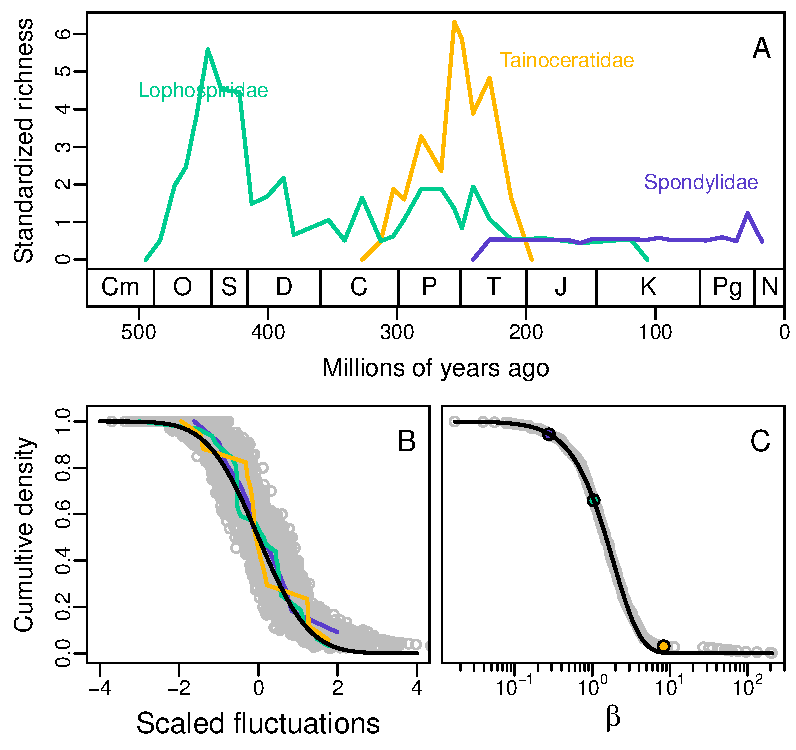
\includegraphics[scale=0.8]{../../fig_pkx-fbeta.pdf}
  \caption[Variability in trajectories of within-order fluctuations in
  genus richness]{The distributions of within-order fluctuations in
    genus richness shown for the trajectories of three exemplar
    orders (A) and shown as an empirical cumulative density aggregated
    across all orders (B). To display all orders simultaneously we
    simply collapse their fluctuation distributions by dividing by
    their standard deviations. If orders conform to the Gaussian
    hypothesis their scaled fluctuations should fall along the
    cumulative density line of a normal N(0, 1) distribution, as shown
    in (B). In (C) the distribution of inverse variances $\beta_k$
    across all orders matches very closely to a Gamma distribution
    (black line); exemplar orders are again highlighted.}
  \label{fig:pk_f}
\end{figure}


To predict the super-statistical behavior of the entire marine
invertebrate Phanerozoic fauna we must integrate over all possible
local equilibria that each clade could experience. The stationary
distribution of $\beta_k$ values describes these possible equilibria,
specifying the probability that a given clade, chosen at random, will
occupy a region of adaptive space characterized by $\beta_k$.

%%% move elsewhere if not said already
% The form of
% this stationary distribution could shed interesting light on the
% biological processes that lead different clades to explore different
% regions of adaptive landscapes, and thus different equilibria, as
% discussed below.
%%%

We estimate the distribution of $\beta_k$'s simply as the maximum
likelihood distribution describing the set of volatilities for all
families, orders, classes, or phyla. Phanerozoic marine invertebrate
families clearly follow a Gamma distribution in their $\beta_k$ values
(Fig. \ref{fig:pk_f}). This Gamma shape also holds for orders and
shows increasing deviations again for classes and especially phyla
(Fig. \ref{figSupp:fbeta_allTaxa}).

Using the observation of within family statistical equilibrium and
Gamma-distributed $\beta_k$ parameters we can calculate, without
further adjusting free parameters, the distributions of family-level
fluctuations for the entire marine Phanerozoic, $P(x)$, as
\begin{equation}
  P(x) = \int_0^\infty p_k(x \mid \beta) f(\beta) d\beta \label{eq:PxInt}
\end{equation}
where
$p_k(x \mid \beta) = \sqrt{\frac{\beta}{2\pi}} e^{-\frac{\beta
    x^2}{2}}$ is the distribution of fluctuations within an order and
$f(\beta) = \frac{1}{\Gamma(b_1/2)}
\left(\frac{b_1}{2b_0}\right)^{b_1/2} \beta^{(b_1/2) - 1}
\text{exp}\left(-\frac{b_1 \beta}{2 b_0}\right)$ is the stationary
distribution of volatilities in richness fluctuations. The integral in
(\ref{eq:PxInt}) leads to
\begin{equation}
  \label{eq:Px}
  P(x) = \frac{\Gamma\left(\frac{b_1 +
        1}{2}\right)}{\Gamma\left(\frac{b_1}{2}\right)}
  \sqrt{\frac{b_0}{\pi b_1}} \left(1 + \frac{b_0
      x^2}{b_1}\right)^{-\frac{b_1 + 1}{2}}
\end{equation}
This corresponds to a non-Gaussian, fat-tailed prediction for $P(x)$
which closely matches aggregated family level fluctuations in the
bias-corrected PBDB (Fig. \ref{fig:Px}).

\begin{figure}[!h]
  \centering
  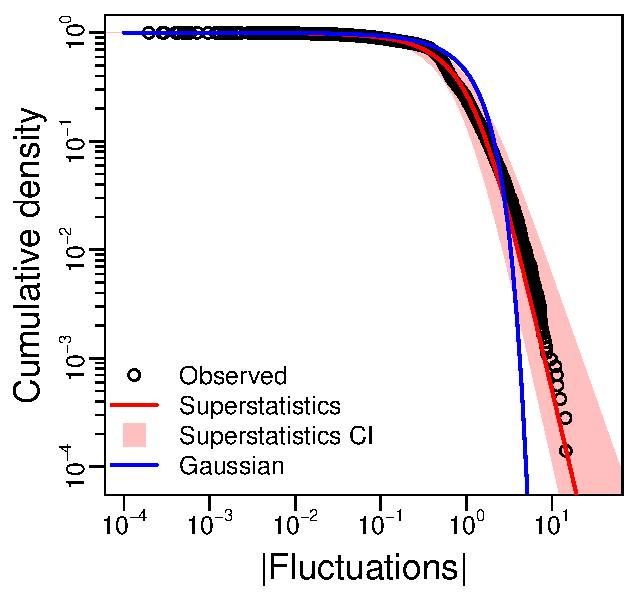
\includegraphics[scale=1]{../../fig_Px.pdf} 
  \caption[Order-level distribution of richness
  fluctuations]{Distribution of fluctuations in genus richness within
    orders of marine invertebrates in the Paleobiology Database
    \citep{alroy08} after sampling correction. The distribution is
    fat-tailed as compared to the maximum likelihood estimate of the
    normal distribution (blue line).  At the order level the empirical
    distribution of fluctuations are well described by our
    super-statistical approach, both when computed from integrating
    over the distribution of observed variances (red line) and when
    fit via maximum likelihood (95\% confidence interval; red
    shading).}
  \label{fig:Px}
\end{figure}

To quantitatively evaluate how well the super-statistical prediction
matches the family-level data we constructed a 95\% confidence
envelope from bootstrapped maximum likelihood estimates for
$P(x)$. Observed fluctuations fall within this 95\% confidence
envelope (Fig. \ref{fig:Px}), indicating that the data do not reject
the super-statistical prediction. For further comparison, we fit a
Gaussian distribution to the observed fluctuations, which corresponds
to the equilibrium hypothesis that all orders conform to the same
dynamic. Using Akaike Information Criterion (AIC) we find that
observed fluctuations are considerably better explained by the
super-statistical prediction than by the Gaussian hypothesis ({\small
  $\Delta$}AIC = 1895.622). Thus, as expected under the
superstatistical hypothesis, the fat-tailed distribution of
fluctuations arise from the superposition of independent Gaussian
statistics of fluctuations within families.

%% calculating sstat at different taxonomic levels (D-stat fig)
Computing the distribution of aggregated fluctuations using orders
also closely matches the observec data (Fig. \ref{fig:Px}) but as we
further coarsen the taxonomy to classes and phyla we see increasingly
poorer correspondance between data and theory (Fig. \ref{fig:Px}). We
quantify this change in the goodness of fit with the
Kolmogorov-Smirnov statistic (Fig. \ref{fig:dStat}). We can see that
both families and orders have low Kolmogorov-Smirnov statistics, and
in fact order level designation of equilibrial subsystems performs
slightly better than the family level. Classes are substantially worse
and phylo worse yet with the Kolmogorov-Smirnov statistic of phyla
being no different than the null randomized taxonomies described
below.

However, if super-statistical theory explains the data, this worsening
fit with increasing taxonomic scale is expected as the different
classes and phyla should not represent dynamically equilibrial
sub-systems in their fluctuation dynamics. Instead, classes and phyla
aggregate increasingly disparate groups of organisms, and thus
effectively mix their associated Gaussian fluctuations, meaning that
one statistic should no longer be sufficient to describe class-level
dynamics. We see this confirmed by the increasing frequency of outlier
fluctuations in within class and phylum level fluctuation
distributions (Fig. \ref{figSupp:pkx_allTaxa}). We can also see that
families and orders represent, on average, 1 to 2 Bambachian ecospace
hypercubes \citep{bambach}, respectively, in contrast to classes and
phyla which represent, on average, 8 to 30 hypercubes, respectively
(Fig. \ref{figSupp:eeSpaceOcc}).


Our analysis indicates that orders and families are evolutionarily
coherent units with all subsumed taxa sharing key ecological
and evolutionary attributes allowing them to reach steady state
diversification independently from other clades at global scale. The
fact that both orders and families conform to theoretical predictions
is consistent with superstatistics. If superstatistics operates at the
order level, then the families subsumed by these orders should
represent random realizations of their order's stationary $\beta_k^{(order)}$
volatility. The sum of Gamma random variables is still Gamma, but with
new parameters, thus the family level distribution of
$\beta_k^{(family)}$ is still Gamma.

\begin{figure}[!h]
  \centering
  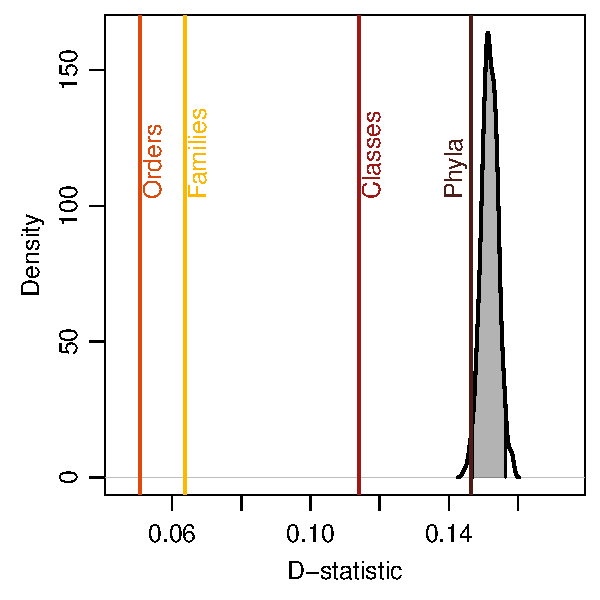
\includegraphics[scale=1]{../../fig_dStat.pdf}
  \caption[Goodness of super-statistical theory fit]{Distribution of
    Kolmogorov-Smirnov (KS) statistics from randomly permuting genera
    within orders (gray shading represents 95\% confidence
    interval). Solid black line is observed KS statistic at the order
    level, while the dashed black line shows the observed KS statistic
    at the class level.}
  \label{fig:dStat}
\end{figure}

To further test the evolutionary coherence of families we conducted a
permutation experiment in which genera were randomly reassigned to
families while maintaining the number of genera in each family. For
each permutation, we calculated the super-statistical prediction and
its Kolmogorov-Smirnov statistic. The permutation simulates a null
model in which common evolutionary history is stripped away (genera
are placed in random families) but the total number of observed genera
per family is held constant, thus controlling for the distribution of
genera per family which could result from arbitrary taxonomic
desicions \citep{YuleSomething}.  Repeating this permutation 500 times
yields a null distribution of Kolmogorov-Smirnov statistics that is
far separated from the observed values at the family and order levels
(Fig. \ref{fig:dStat}) suggesting the good fit at these levels is not
merely a statistical artifact of classification but carries important
biological information. It should also be noted that the width of 95\%
confidence interval of this null distribution is not far from the
distance between the Kolmogorov-Smirnov statistics of orders versus
families, suggesting that differences of fit between these taxonomic
levels is at least partially accounted for by the randomness of the
sampling distribution of Kolmogorov-Smirnov statistics.

\section{Discussion}

%% why orders
Our analysis makes no assumption that orders and families should
correspond to super-statistical subsystems, but identifies them as the
appropriate level for marine invertebrates. As we show, orders and the
families they subsume differ only in the volatilities of their
richness fluctuations (Fig. \ref{fig:pk_f}).

Our study is the first to demonstrate that complex patterns in the
fluctuation of taxon richness in the fossil record are the result of a
simple underlying process analogous to the statistical mechanisms by
which complexity emerges in large, non-equilibrium physical
\citep{beck2004} and social systems \citep{fuentes2009}.  We do so by
identifying the biological scale at which clades conform to locally
independent dynamic equilibria in fluctuations.  Equilibrium could
result from many processes, including neutrality \citep{macWilson,
  hubbell2001, olszewski2004}, diversity-dependence
\citep{rabosky2009ecolLett, moen2014, foote2018} and processes that
dampen---rather than exacerbate---fluctuations in complex ecological
networks \citep{berlow2009}. These candidate processes are directly
opposed to the instability hypothesis underlying the self-organized
criticality hypothesis for paleo biodiversity \citep{bak1993,
  sole1997}.

We show the distribution describing the evolution to different
equilibria between orders is Gamma (Fig. \ref{fig:pk_f}).  A Gamma
distribution, while consistent with multiple processes (e.g.,
\citep{cir1985}), could result from evolution of diversification rates
across an adaptive landscape that promotes niche conservatism and
pulsed exploration of niche space.  Specifically, if $\beta_k$ values
are associated with a clade's macroevolutionarily-relevant traits, and
those traits evolve via Ornstein-Uhlenbeck-like exploration of an
adaptive landscape, the resulting stationary distribution of $\beta_k$
will be Gamma \citep{cir1985, butler2004}.  For macroevolutionary
rates to vary across an adaptive landscape, this landscape cannot be
flat, and thus niche conservatism interrupted by adaptive exploration
is likely \citep{newman1985adaptive, gavrilets2004book}. The specifics
of how this adaptive landscape is shaped and is traversed by evolving
clades determine the exact form of the distribution of $\beta_k$
volatilities, in the case of the marine Phanerozoic resulting in a
Gamma. Our work thus motivates further study of the trait spaces and
evolutionary shifts consistent with Gamma-distributed equilibria in
richness fluctuation volatilities.

We then show that the pulsed shift to different equilibria between
orders and the families they subsume is sufficient to explain the
characteristically fat-tailed distribution of richness fluctuations
when the marine Phanerozoic fauna is viewed as a whole macrosystem.
Armed with an understanding of the statistical origin of this
diversification pattern we can explore which models of niche
conservatism and pulsed adaptive radiation in are consistent with the
statistical behavior of the Phanerozoic. Our statistical theory
provides new motivation for identifying the eco-evolutionary causes of
innovations between lineages and how those innovations are eventually
conserved within lineages. With a theoretical baseline, we can also go
on to identify and robustly examine the mechanisms underlying patterns
unexplained by our statistical theory. For example, clades wax and
wane systematically, and possibly non-symetrically, through time
\citep{liow2007, foote2008paleobiol, quental2013}, a pattern that we
cannot explain with superstatistics alone.

%% note on how sstat could be applied to other questions in eco-evo.
Superstatistics could also be applied to other areas of evolution and
macroecology.  For example new phylogenetic models already consider
heterogeneous rates of diversification (e.g.,
\citep{rabosky2014}). The superstatistics of clades in adaptive
landscapes could motivated models that jointly predict changes in
trait and diversification, a research area currently strugelling with
model inadequecy \citep{rabosky2017fisse}. This framework could also
provide a new paradigm in modeling the distributions of richness,
abundance and resource use in non-neutral communities. Non-neutral
models in ecology are criticized for their over-parameterization
\citep{rosindell2011}, yet a persistent counter argument to neutral
theory \citep{hubbell2001} is the unrealistic assumption of ecological
equivalency \citep{chave2004neutral} and poor prediction of real
dynamics \citep{ricklefs2006neutral}. If ecosystems are viewed as the
super-position of many individualistically evolving clades, each
exploiting the environment differently and thus obeying a different
set of non-equivalent statistics, then diversity dynamics could be
parsimoniously predicted with superstatistics while incorporating real
biological information on ecological differences between taxa.

Superstatistics is a powerful tool to derive macro-scale predictions
from locally fluctuating sub-systems whose evolution is driven by
interesting, but complex and difficult to model, biological
mechanisms. As such, applications of superstatistics from islands to
populations to clades are ripe for exploration.


\section{Methods and Materials}

All data processing and analyses were preformed in R \citep{rcite} and
all code needed to reproduce our study are provided, with added
explaination, in the supplement.

\subsection{Paleobiology Database data download and filtering}
Data were downloaded from the Paleobiology Database (PBDB; {\tt
  https://paleobiodb.org}) on 16 November 2018 via the database's API
(data retrival and processing script in the supplement). Collections
were filtered using the same approach as Alroy \citep{alroy08} to
insure that only well preserved marine invertebrate occurrences were
used in subsequent analyses. This filtering resulted in 815,222 unique
genus-level occurrences. These were further filtered to exclude those
occurrences without family-level taxonomy and those collections with
age estimate resolutions outside the 11MY timebins proposed by Alroy
\citep{alroy08} resulting in 454,033 occurrences. These timebins were
compiled from {\tt http://fossilworks.org} with a custum script
reproduced in the supplement. The first and last of these timebins,
corresponding to the earliest Cambrian and the latest Cenozoic, were
excluded from analysis because their sampling completeness (see below)
could not be assessed.


\subsection{Correcting for imperfect and potentially biased sampling}
\label{sec:3TP}
We use a new and flexible method to correct for known sampling
incompleteness and biases in publication-based specimen databases
\citep{alroy08, alroy2010}. Incompleteness is inherent in all
biodiversity samples, the fossil record being no exception
\citep{miller1996, foote2016, starrfelt2016, close2018}. This
incompleteness is only an issue if it varies across the fossil record,
as indeed it does \citep{miller1996 , foote2016, starrfelt2016,
  close2018}.  In addition to variable incompleteness, bias may result
from preferential publication of novel taxa \citep{alroy2010} which
exacerbates the difference between poorly-sampled and well-sampled
time periods. We therefore develop a simple two-step method: we first
correct genus richness for incomplete sampling using the
``three-timer'' correction \citep{alroy08} and then further correct
this three-timer richenss estimate by accounting for any correlation
between the number of genera and the number of publications in a time
period.

The three-timer correction estimates the probability of failure to
observe a genus in a given time period $p_t$ as the number of times
any genus is recorded before and after that period but not during,
divided by the number of genera whoes occurrence histories span the
period $t$.  To calculate the sampling-corrected richness
$\hat{D}_{kt}$ of a clade $k$ in the time period in question, the
observed genera within that clade and time period are divided by
$1 - p_t$ and their occurrences summed:
\begin{equation}
  \hat{D}_{kt} = \sum_{j \in k} \frac{I_{jt}}{1 - p_t}
\end{equation}
where $j \in k$ designates genera in clade $k$ and $I_{jt}$ is an
indicator equal to 1 if genus $j$ occurs in time period $t$.

$\hat{D}_{kt}$ is the maximum likelihood estimator of richness in a
simple occupancy through time type model assuming binomial sampling
\citep{royleDorazio}, and in that way mimics other proposed methods
for the fossil record \citep{foote2016, starrfelt2016}. We avoid
parametrically modeling the sampling process through time by instead
taking a sliding window of timebins from the Cambrian to the
Cenozoic. It should be noted that the three-timer correction compares
favorably to other similar methods to account for imperfect detection
\citep{alroy2014}

To eliminate further bias due to preferential publication of novel
taxa \citep{alroy2010} we divide the three-timer-corrected number of
genera per family per time period by the expected number of genera
given publications in that time period.  The expected number is
calculated by regressing the log-transformed three-timer-corrected
number of genera on log-transformed number of publications. There is
only a weak trend toward higher richness with more publications
(Fig. \ref{fig:divByPub}) meaning that the most important correction
comes from the three timer correction.

Our new method re-scales each genus occurrence from 0 or 1 (absent or
present) to a weighted number continuously ranging between 0 and
1. Because these weighted numbers represent sampling and
bias-corrected {\it occurrences} we can add them arbitrarilly,
corresponding to the membership of any given genus in any given higher
taxonomic group.  We must, however, choose a taxonomic level at which
to evaluate the relationship between richness and publications; we
choose the level of family because this is the most finely resolved
option.

We opt not to use subsampling methods \citep{miller1996, alroy2010,
  kocsis2018} because these approaches would not be advisable for
clades with few genera. However, our new method achieves similar
results at the global scale across all clades to subsampling
procedures. We directly compare our predicted time series of global
fluctuations in genus richness with results derived from rarifaction
and shareholder quarum subsampling (SQS) in Figure
\ref{fig:supp_3TPub}.  Our method shows very minor differences with
these subsampling-based predictions and any discrepancies do not
impact the statistical distribution of fluctuations
(Fig. \ref{fig:supp_3TPub}).


\subsection{Super-statistical methods} \label{sec:numMeth}

We first derive the super-statistical distribution $P(x)$ by fitting
Gaussian distributions to clade-level distributions of fluctuations
$p_k(x)$, extracting the inverse variances $\beta_k$ of those
$p_k(x)$, testing the best function to describe the distribution of
$\beta_k$, and then integrating
$P(x) = \int_{\beta}p_k(x | \beta) f(\beta)$. This process allows no
free parameters to hone the fit of $P(x)$ to the data.  However, each
inverse variance must of course be estimated for each clade, making
its good fit to data all the more surprising.  To do so we use least
squares instead of maximum likelihood because the asymmetric
fluctuation distributions of small clades were more reliably fit with
curve fitting than with maximum likelihood.

We then estimated $P(x)$ directly from the raw data using maximum
likelihood to compare the fit of our super-statistical prediction and
that of a simple Gaussian distribution using AIC. To calculate a
likelihood-based confidence interval on our prediction we bootstrapped
the data, subsampling fluctuations with replacement from all families
and fit superstatistics using maximum likelihood to the aggregated
fluction distribution of each bootstrap replicate.

\bibliographystyle{Science}
\bibliography{../../superStat}


\section*{Acknowledgments}
\begin{itemize}
\item[{\bf General:}] We thank John Harte, Rosemary Gillespie, Linden
  Schneider, Jun Ying Lim, and David Jablonski for helpful
  discussion. We thank the many contributors to the Paleobiology
  Database for making data available.
\item[{\bf Funding:}] AJR thanks funding from Fulbright Chile, the
  National Science Foundation Graduate Research Fellowship Program and
  the Omidyar Program at the Santa Fe Institute; MAF thanks FONDECYT
  1140278; PM thanks CONICYT PFB-023, ICM-P05-002 and FONDECYT
  1161023.
\item[{\bf Author contributions:}] AJR, MAF and PAM designed the
  study; AJR and MAF preformed the analyses; AJR, MAF and PAM
  interpreted the results and wrote the manuscript.
\item[{\bf Competing interests:}] none.
\item[{\bf Data and materials availability:}] Data are available
  through the Paleobiology Database ({\tt paleobiodb.org}) and all
  code needed to interface with the {\tt paleobiodb.org} API, process,
  clean, and ultimately analyze the data are available online at {\tt
    github.com/ajrominger/paleo\_supStat}. This github repository also
  hosts the exact download from {\tt paleobiodb.org} used in this
  analysis. All required scripts are also availible and explained in
  the Supplement.
\end{itemize}


\clearpage

\newcommand{\beginsupplement}{%
  \setcounter{table}{0}
  \renewcommand{\thetable}{S\arabic{table}}%
  \setcounter{figure}{0}
  \renewcommand{\thefigure}{S\arabic{figure}}%
  \setcounter{section}{0}
  \renewcommand{\thesection}{S\arabic{section}}%
}

\beginsupplement

\begin{center}
{\LARGE \bf Supplementary materials}
\end{center}
\vspace{2em}

\section{Limit distribution of a time-averaged homogeneous
  origination-extinction process}
\label{sec:suppLimitDist}

Fossil taxa gain and lose genera according to an origination-extinction
process. We assume that most fossil occurrences of a taxon come from
the period of its history when it is dominant and in steady state. In
a time slice of duration $\tau$ during such a period of steady state
the latent per capita rates of origination and extinction would be
equal (i.e. $\lambda = \mu \equiv \rho$) and the number of origination
or extinctions events (call such events $Y$) each follow an
inhomogeneous Poisson process with rate $\rho N_t$ where $N_t$ is the
number of species or genera in the taxon of interest at time
$t$. Allowing $N_t$ to vary smoothly with time, and recognizing that
the sum of Poisson random variables remains Poisson, we arrive at the
number $Y$ of extinction \emph{or} origination events in $\tau$ being
distributed
\begin{equation}
  \label{eq:eventPois1}
  Y \sim \text{Pois}(\rho \int_{t=0}^\tau N(t) dt).
\end{equation}
Under the steady state assumption we can approximate $N(t)$ by
$\bar{N}$, the steady state richness, leading to
\begin{equation}
  \label{eq:eventPois2}
  Y \sim \text{Pois}(\rho \bar{N} \tau).
\end{equation}

This Poisson distribution is asymptotically Gaussian, which is a more
appropriate distribution for our sampling and bias-corrected richness
estimates because these estimates are not integer-valued but rather
continuous random variables. Furthermore, because we ue standard time
periods of average duration $\tau = 11\text{MY}$ the the distribution
of fluctuations within taxa will be independent of the specific time
periods considered. The Gaussian asymptotics of time-averaged
birth-death processes have been proven and explored elsewhere as well
\citep{keilson1970, grassmann1987}.


\section{Evaluation of sampling bias correction methods}
\label{sec:suppBiasEval}

\citep{kocsis2018}

\begin{figure}[!hp]
  \centering
  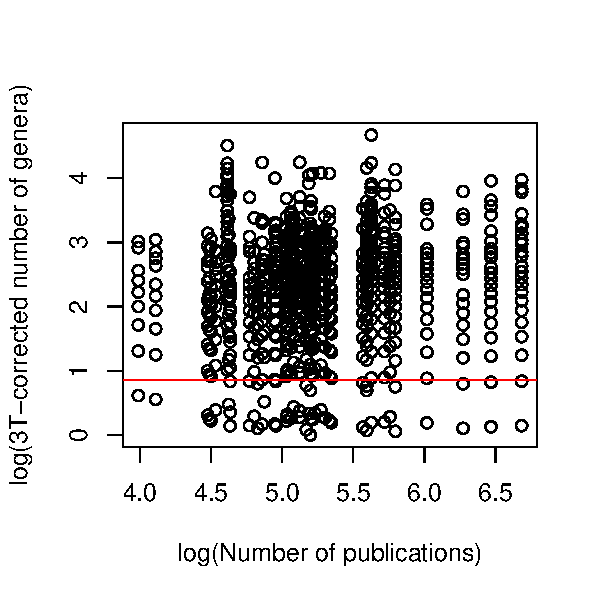
\includegraphics[width=0.4\textwidth]{../../figSupp_divByPub.pdf}
  \caption[Relationship between number of publications and genus
  richness]{Relationship between number of publications and genus
    richness as recorded by the PBDB.}
  \label{fig:divByPub}
\end{figure}

\begin{figure}[!hp]
  \centering
  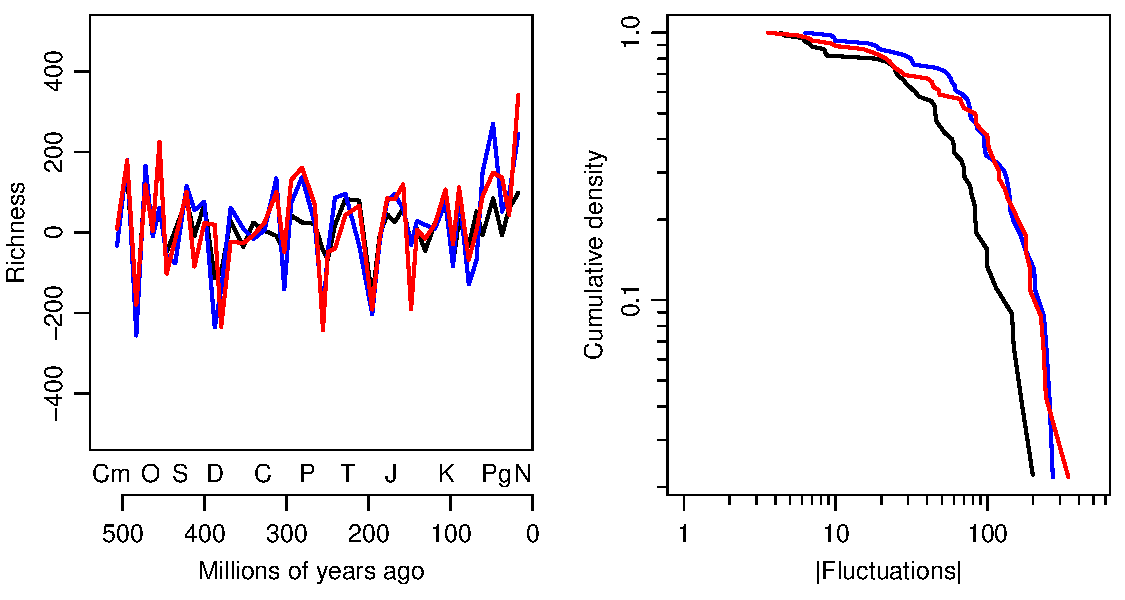
\includegraphics[width=0.7\textwidth]{../../figSupp_divEstComp.pdf}
  \caption[Comparison of SQS method with the raw data and three-timer
  bias correction method]{Comparison of SQS method \citep{alroy2010}
    (solid black line) with the raw data (dashed black) and our
    three-timer and publication bias correction method (red). The
    time-series of all marine invertebrate genera shows general
    agreement with the only major deviations toward the modern
    (A). Despite these differences the distribution of fluctuations in
    genus richness across all marine invertebrates show good
    agreement (B).}
  \label{fig:supp_3TPub}
\end{figure}


\section{Understanding deviations from superstatistics at higher
  taxonomic levels}
\label{sec:suppSstatTaxLevels}


\section{Guild composition of higher taxa}
\label{sec:suppGuilds} 

\begin{figure}[!hp]
  \centering
  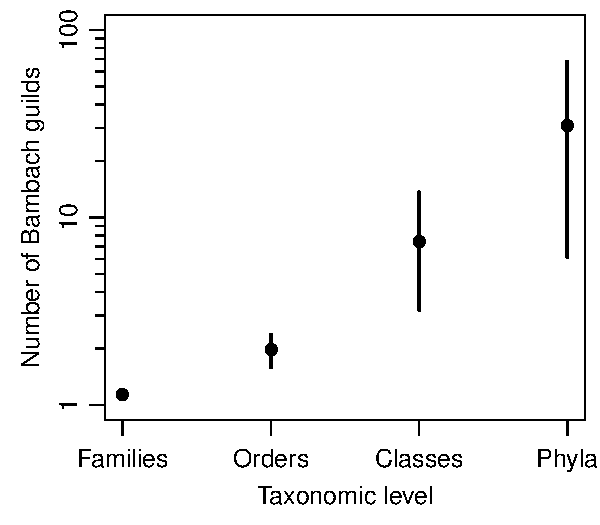
\includegraphics[width=0.4\textwidth]{../../figSupp_eeSpaceOcc.pdf} 
  \caption[Relationship between number of Bambachian guild hypercubes
  and taxonomic level]{Relationship between number of Bambachian guild hypercubes
  and taxonomic level.}
  \label{figSupp:eeSpaceOcc}
\end{figure}

\end{document}

